\section{Nome do Jogo}
%Colocar duas citações diretashack 
Ogof e o templo das joias.

\section{\textit{High Concept} do Jogo}
Ogof e o templo das joias é um game de fantasia, em que o jogador assumirá o papel de 3 diferentes figuras, e trabalhar em conjunto para progredir.
% Ogof e o templo das joias é um game de fantasia, exploração e puzzle em que você irá assumir o papel de 3 figuras de diferentes épocas do tempo, 
% % cada qual com suas forças e fraquezas, para progredir será necessário explorar as forças de cada personagem
% e trabalhar em conjunto para descobrir os planos de Ogof.

% Conceito em 150 caracteres


\section{Gênero}

O jogo será 3D em terceira pessoa, com fases que irão misturar diversas mecânicas como \textbf{puzzle, hack em slash} e exploração. Cada fase será linear com a dificuldade gradualmente aumentada até o final da fase, em que cada uma terá um miniboss.

% Descreva e justifique o genero do jogo

\section{Púbico Alvo}

% Descreva e justifique o publico alvo do jogo
Adolescentes a partir de 16 anos....
\vfill
\pagebreak

\section{\textit{Game Flow}}
\begin{figure}[!htb]
	\caption{\label{fig_grafico}Fluxo de telas}
	\begin{center}
	    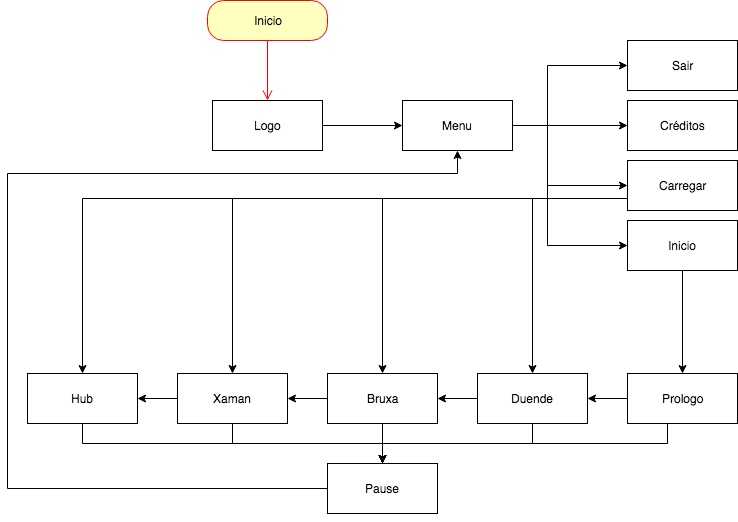
\includegraphics[width=\textwidth]{imagens/Flow.png}
	\end{center}
	\legend{Fonte: Própria Autoria}
\end{figure}
Ilustração ou tabela que monstre todas as telas que o jogo terá e como se relacionam entre si

\section{Estilo estético}
De acordo com Ethan Redd desenvolvedor, designer e palestrante do seminário "Low Poly Modeling: Style Through Economy" na GDC: "Low poly is what I like to call quantifiabiably qualitative. There's no hard definition for it, but I like to think of it as the discipline and aesthetic of surface economy. So basically describing 3D or sometimes 2D surfaces as little geometry as necessary to get the idea across it"  ("Low poly é o que eu gosto de chamar de quantificável qualitativamente. Não é um conceito complicado, eu gosto de pensar nela como uma disciplina e estética de economia de superfície. Basicamente, podemos descrevê-lo como superfícies 3D ou ocasionalmente 2D com o mínimo de geometria necessária para transmitir uma ideia" [tradução própria]) .

Decidimos trabalhar com low poly porque demanda menos processamento e tempo de renderização, sendo assim mais amigável aos nossos equipamentos e aos dos nossos usuários em potencial. Além de ter uma modelagem mais fácil --sendo muito adequado ao tempo de que dispomos -- e ser visualmente divertido, tendo em vista que visamos atingir o público no início da adolescência. 

\begin{figure}[!htb]
	\caption{\label{LowPoly}Low Poly}
	\begin{center}
	    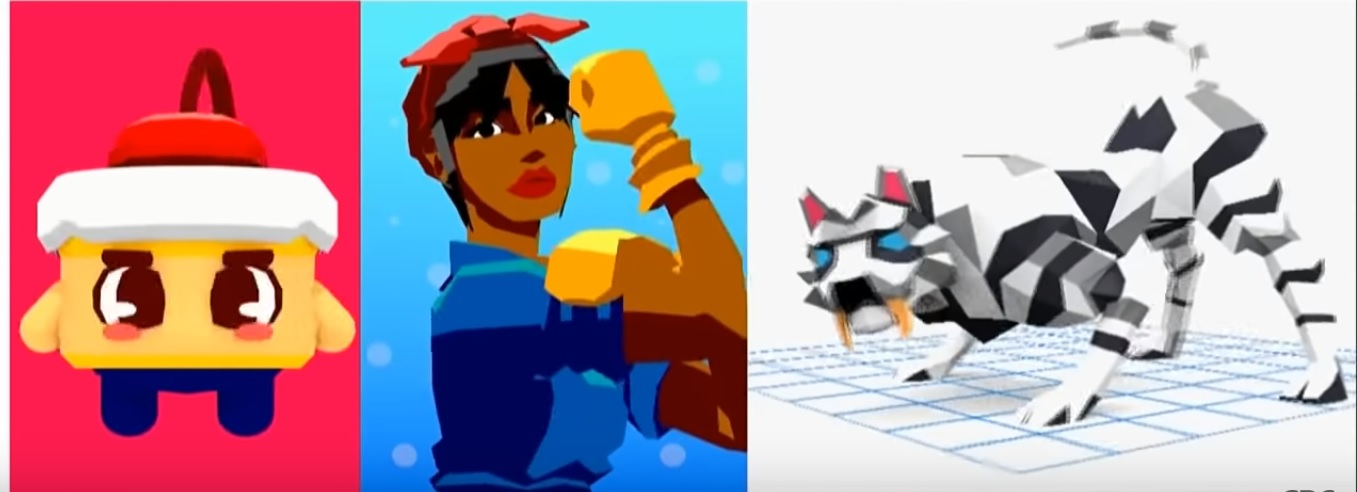
\includegraphics[width=\textwidth]{imagens/lowPoly.jpg}
	\end{center}
	\legend{Fonte: "Low Poly Modeling: Style Through Economy"  palestrado por Ethan Redd na GDC}
\end{figure}


\clearpage
\section{Inspirações}

\subsection{Outlander}

Em 1945, em lua de mel na Escócia, a enfermeira em combate Claire Randall é misteriosamente transportada através do tempo para o ano de 1743.

\begin{figure}[!htb]
	\caption{\label{Outlander}Outlander}
	\begin{center}
	    
\includegraphics[width=0.3\textwidth]{imagens/outlander.jpg}
	\end{center}
	\legend{Fonte: Diana Gabaldon - 1991}
\end{figure}

\subsection{Filha de Feiticeira}

Este romance de Celia Rees narra, em forma de diário, a história de Mary Nuttall, uma adolescente inglesa do século XVII que se vê obrigada a fugir para a América para não ter o mesmo destino de sua avó, condenada à forca sob acusação de feitiçaria.

\clearpage

\begin{figure}[!htb]
	\caption{\label{Filha de Feiticeira}Filha de Feiticeira}
	\begin{center}
	    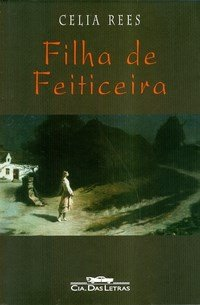
\includegraphics[width=0.3\textwidth]{imagens/feiticeira.jpeg}
	\end{center}
	\legend{Celia Rees - 2002}
\end{figure}



\subsection{Desencanto}

Bean é uma princesa que vive no reino mágico de Dreamland ao lado de Luci, seu demônio pessoal, e de Elfo, seu melhor amigo que a acompanham em sua jornada de alcoolismo, brigas de bar e descobertas inusitadas.



\begin{figure}[!htb]
	\caption{\label{Desencanto}Desencanto}
	\begin{center}
	    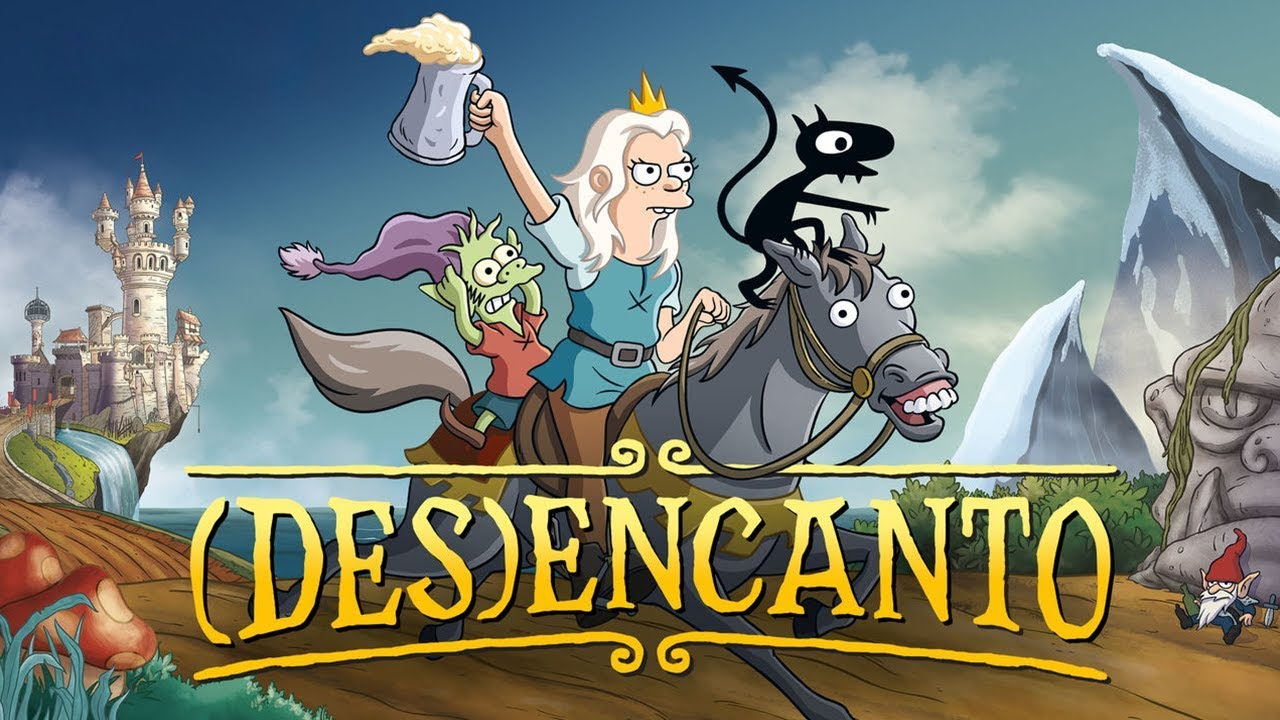
\includegraphics[width=\textwidth/2]{imagens/Desencanto.jpg}
	\end{center}
	\legend{\cite{dessencanto}}
\end{figure}

\subsection{Os Vingadores - Guerra infinita}

Inspirou a proposta de coleta de joias e a personalidade de Ogof teve referência no personagem Thanos.

\begin{figure}[!htb]
	\caption{\label{vingadores}Poster do Filme}
	\begin{center}
	    
\includegraphics[width=0.3\textwidth]{imagens/vingadores.jpeg}
	\end{center}
	\legend{\cite{avengers}}
\end{figure}

\subsection{Franquia God of War}

Sinopse:

Inspirou a animação, técnica de câmera e combate do gameplay.


\begin{figure}[!htb]
	\caption{\label{god_of_war}God of War}
	\begin{center}
	    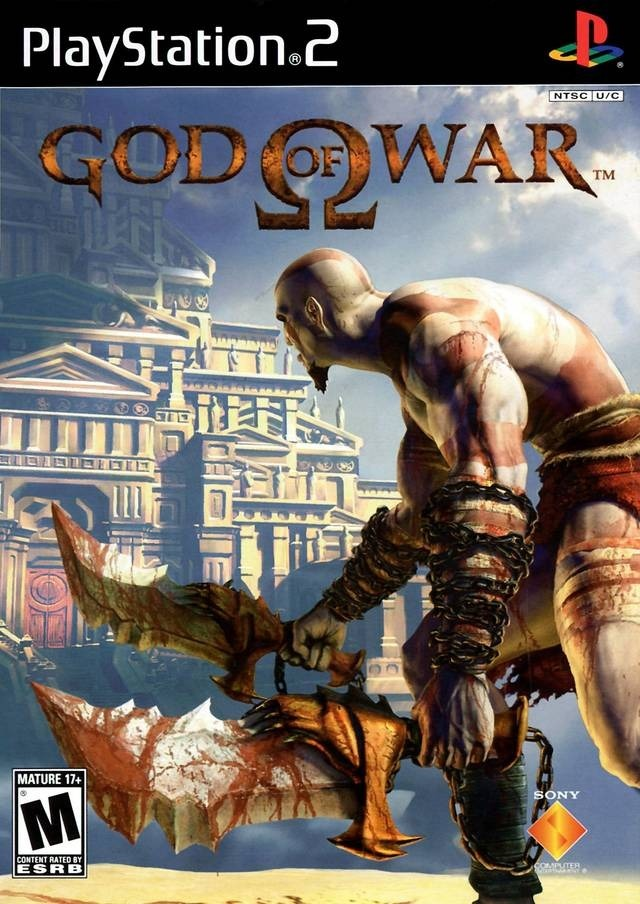
\includegraphics[width=0.3\textwidth]{imagens/GodofWar.jpg}
	\end{center}
	\legend{\cite{godofwar}}
\end{figure}

\clearpage

\subsection{Sonhos de uma noite de verão}

Sinopse:


\begin{figure}[!htb]
	\caption{\label{sonhos_shakespeare} Capa Sonhos de uma noite de Verão}
	\begin{center}
	    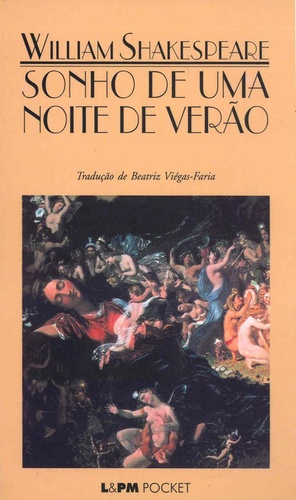
\includegraphics[width=0.3\textwidth]{imagens/Sonhos.jpg}
	\end{center}
	\legend{L\&PM Pocket, William Shakespeare - 1605}
\end{figure}


\subsection{Brownies}

Brownies são pequenos seres noturnos do folclore britânico, que cuidam dos afazeres da casa, se ofendem facilmente e evitam serem vistos pelos humanos \cite{britannica_2011}\cite{carolyn_2016}, traços de personalidades que utilizamos como inspiração para a formulação do Duende.
Todo: Inserir as referências na bibliografia, estou tendo dificuldades para achar os livros no formato digital.
\clearpage
\begin{figure}[!htb]
	\caption{\label{fig_brownie}\textbf{Brownie} por Arthur Rackham }
	\begin{center}
	    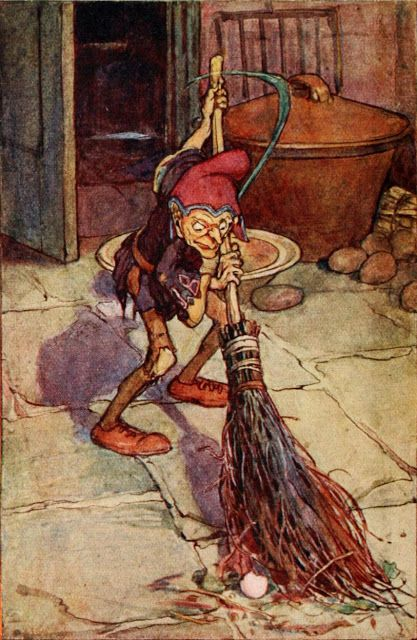
\includegraphics[width=0.3\textwidth]{imagens/brownie.jpg}
		\end{center}
	\legend{William Shakespeare - 1605}
\end{figure}

\subsection{Alux}

Alux são pequenas criaturas da mitologia de alguns povos Maias, costumeiramente são invisíveis, mas podem se tornar visíveis para se comunicar e assustar humanos. Segundo Storniolo (\citeyear{storniolo2009out}) ``When given food, drink, and ritual homage, the aluxo'b protect the farmer’s crops from hungry animals. [...] The aluxo'b summon strong winds, emit piercing whistling sounds, and propel stones at intruders.'' [Quando recebem comida, bebida e um ritual de homenagem, o alux protegerá a plantação do fazendeiro de animais famintos. [...] O alux invoca fortes ventos, emite agudos sons sibilantes, e lança pedras em instrusos: tradução livre]


\begin{figure}[!htb]
	\caption{\label{fig_alux}Alux}
	\begin{center}
	    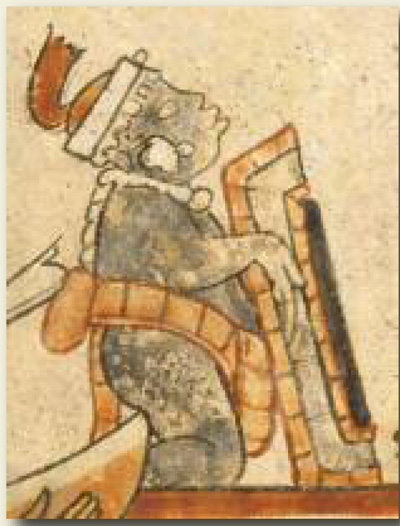
\includegraphics[width=0.3\textwidth]{imagens/alux.jpg}
	\end{center}
	\legend{Fonte:}
\end{figure}


\vfill
\pagebreak

\subsection{Siempre Bruja}

A série que conta a história de uma bruxa negra e escrava que é transportada  pelo tempo para enfrentar um grande bruxo inspirou os poderes da bruxa e itens com os quais trabalha. 

\begin{figure}[!htb]
	\caption{\label{siempre}Siempre Bruja}
	\begin{center}
	    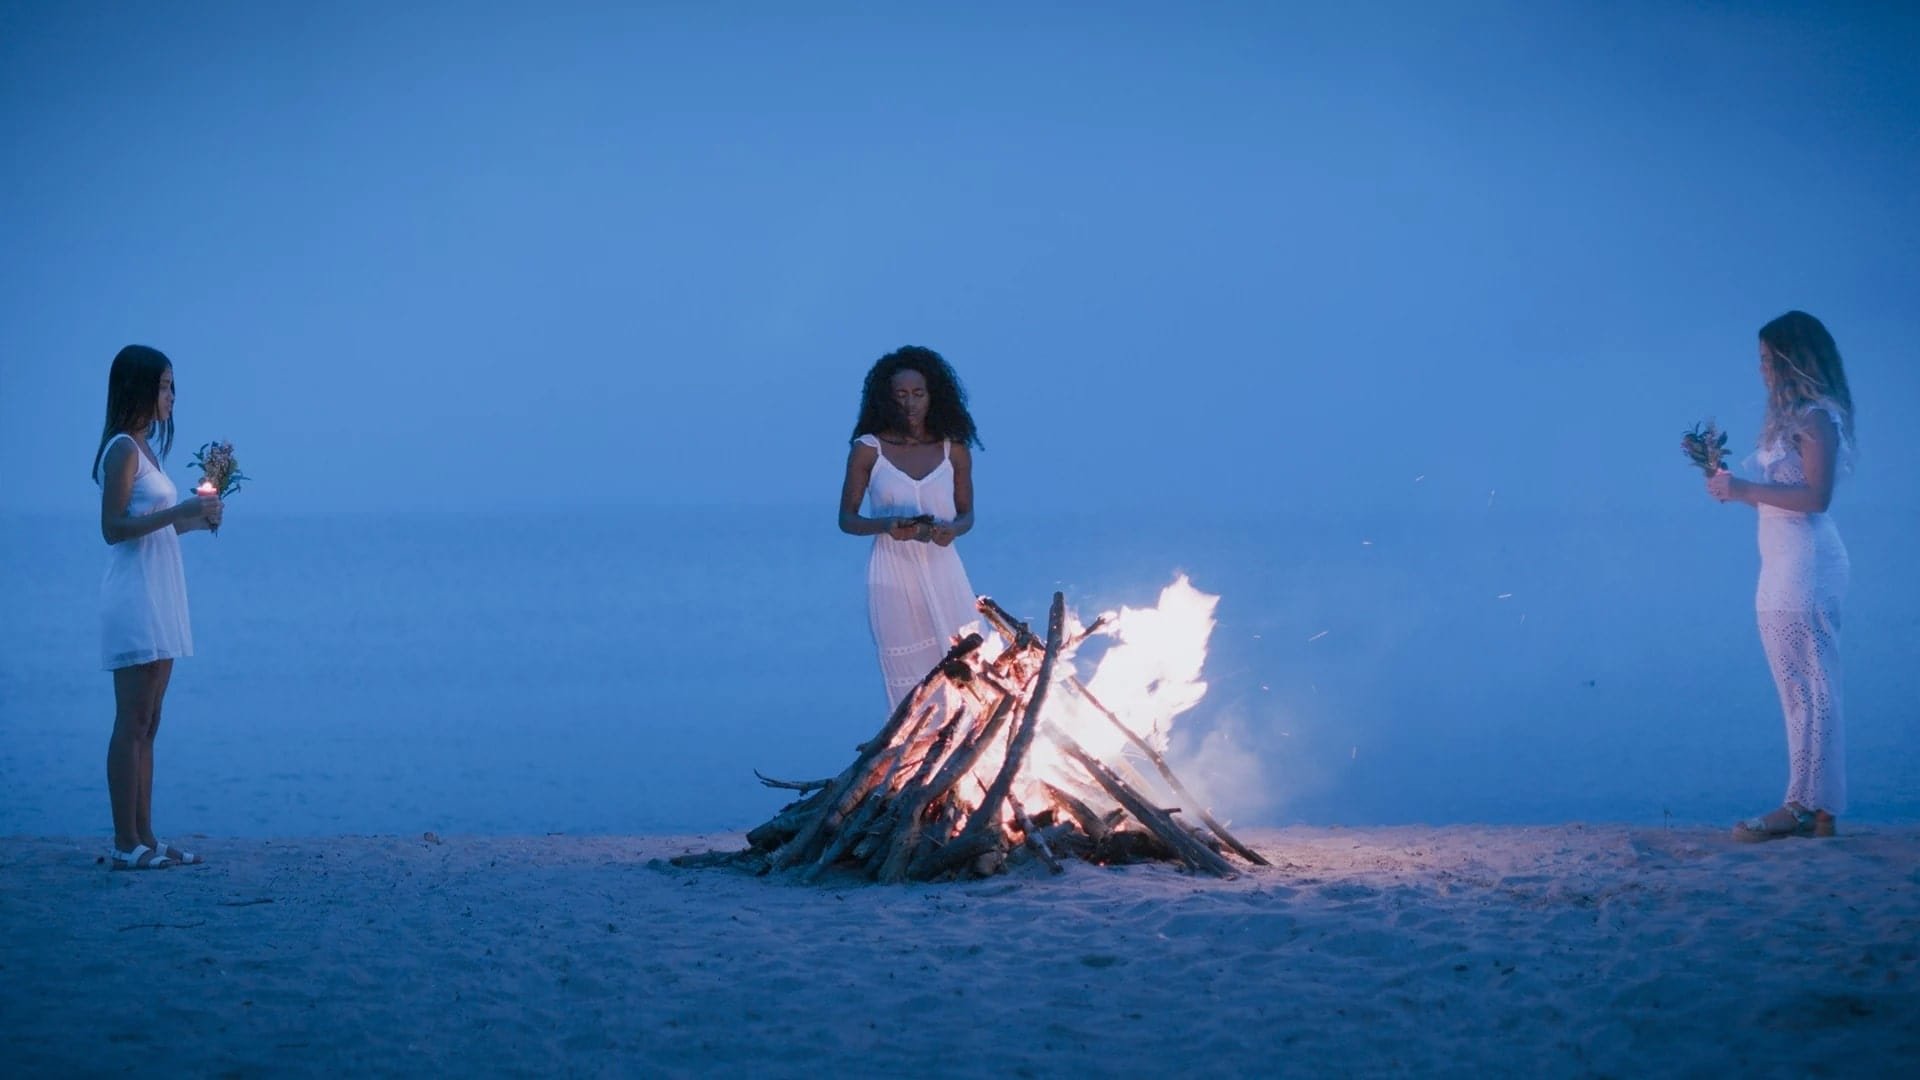
\includegraphics[width=0.5\textwidth]{imagens/SiempreBruja.jpg}
	\end{center}
	\legend{Fonte: }
\end{figure}


\subsection{\textit{The Ghost of a Tale}}
Segundo o site do jogo  "Você é Tilo, um corajoso rato menestrel em uma arriscada missão para achar seu verdadeiro amor. Use sua furtividade e destreza para explorar o Forte \textit{Dwindling Heights}"


\section{Equipe de Desenvolvimento}
Tabelar
A equipe dividiu-se de forma a otimizar as forças de cada um dos integrantes, desta forma ficamos com a seguinte divisão de tarefas não rígidas:

\begin{quadro}[htb]
\caption{\label{quadro_atuacao}Atuação da equipe}
\begin{tabularx}{\textwidth}{|c|X|}
	\hline
	\textbf{Nome} & \textbf{Atuação}\\ \hline
    Marina & Game Design Construção de Personagens, Construção de mundo, Design de personagens, Arte Conceitual \\ \hline
    Eric   & Construção de Personagens, Construção de mundo, Arte Técnica, Programação                                        \\ \hline
    Pedro  & Construção de Personagens, Construção de mundo, Arte Técnica, Programação \\ \hline
\end{tabularx}
\fonte{Propria autoria}
\end{quadro}